\documentclass[12pt, titlepage]{article}

\usepackage{booktabs}
\usepackage{tabularx}
\usepackage{hyperref}
\hypersetup{
    colorlinks,
    citecolor=black,
    filecolor=black,
    linkcolor=red,
    urlcolor=blue
}
\usepackage[round]{natbib}
\usepackage{graphicx}

\input{../Comments}
\input{../Common}

\begin{document}

\title{Verification and Validation Report: \progname} 
\author{\authname}
\date{\today}
	
\maketitle

\pagenumbering{roman}

\section{Revision History}

\begin{tabularx}{\textwidth}{p{3cm}p{2cm}X}
\toprule {\bf Date} & {\bf Version} & {\bf Notes}\\
\midrule
March 9 & 1.0 & Complete document\\
\bottomrule
\end{tabularx}

~\newpage

\section{Symbols, Abbreviations and Acronyms}

\renewcommand{\arraystretch}{1.2}
\begin{tabular}{l l} 
  \toprule		
  \textbf{symbol} & \textbf{description}\\
  \midrule 
  T & Test\\
  \bottomrule
\end{tabular}\\

\wss{symbols, abbreviations or acronyms -- you can reference the SRS tables if needed}

\newpage

\tableofcontents

\listoftables %if appropriate

\listoffigures %if appropriate

\newpage

\pagenumbering{arabic}

This document ...

\section{Functional Requirements Evaluation}

This section reports the evaluation of the functional requirements defined in the
SRS and tested through the system-level procedures introduced in the VnV Plan.
The evaluation focuses on the reimbursement workflow end-to-end: submission,
review and approval, status visibility, receipt persistence, and auditability.

\subsection{Evaluation Approach}

Functional validation was carried out using the planned test cases
\texttt{FRQ-1-SUBMIT}, \texttt{FRQ-2-REVIEW}, \texttt{FRQ-3-STATUS},
\texttt{FRQ-4-STORAGE}, and \texttt{FRQ-5-AUDIT}. Tests combined UI-driven
scenarios, API checks, and database/storage verification to ensure each
requirement was validated through observable behavior and persistent data state.

\subsection{Results Summary}

\renewcommand{\arraystretch}{1.2}
\begin{tabularx}{\textwidth}{>{\raggedright\arraybackslash}p{1.8cm} >{\raggedright\arraybackslash}p{2.0cm} >{\raggedright\arraybackslash}p{2.2cm} X >{\raggedright\arraybackslash}p{1.6cm}}
\toprule
\textbf{Req.} & \textbf{Test ID} & \textbf{Method} & \textbf{Observed Result} & \textbf{Status}\\
\midrule
FRQ-1 & FRQ-1-SUBMIT & UI automation + DB check & Reimbursement requests were submitted successfully with required metadata and receipt links persisted. & Pass\\
FRQ-2 & FRQ-2-REVIEW & UI workflow + backend verification & Reviewer approval/rejection actions updated request state correctly and recorded reviewer decision details. & Pass\\
FRQ-3 & FRQ-3-STATUS & API + UI cross-check & Status values displayed in the dashboard matched API responses and underlying stored state. & Pass\\
FRQ-4 & FRQ-4-STORAGE & Storage/API verification & Uploaded receipts remained retrievable after submission and were protected by role-based access constraints. & Pass\\
FRQ-5 & FRQ-5-AUDIT & Automated log checks & Audit entries were generated for submission and decision events with actor identity and timestamps. & Pass\\
FRQ-6 & FRQ-3-STATUS + role checks & UI/API authorization checks & Access to reimbursement records followed role permissions for submitters, elevated club roles, and MES administrators. & Pass\\
\bottomrule
\end{tabularx}

\subsection{Discussion}

Functional behavior was consistent with the VnV Plan and acceptance criteria.
The highest-risk flow (submission through decision) was validated across multiple
roles and data transitions. In addition, persistence-oriented tests provided
evidence that records and receipt references remained available after workflow
completion, supporting long-term reimbursement traceability.

No critical functional defects were found during the evaluated test scope.
Minor issues related to message clarity and edge-case input feedback are tracked
as implementation refinements and do not block requirement satisfaction.

\section{Nonfunctional Requirements Evaluation}

This section evaluates nonfunctional qualities from the SRS using the planned
test set \texttt{NFL-SAL-1}, \texttt{NFL-USAB-1}, \texttt{NFL-SEC-1}, and
\texttt{NFL-MNT-1}. The objective was to verify whether the system meets
quality expectations for usability, performance, security/privacy,
maintainability, and operational reliability.

\subsection{Usability}

Usability was assessed using task-based sessions aligned with the VnV Plan.
Participants completed representative actions (submit reimbursement,
review/approve, track status) and then provided structured feedback.

\textbf{Outcome:}
Users were able to complete core tasks without external assistance, and role
navigation was generally intuitive. Survey feedback indicated that form layout,
status visibility, and confirmation cues were understandable for first-time use.

\textbf{Assessment:} Pass.
		
\subsection{Performance}

Performance and latency were evaluated through staged load execution on core API
paths and common page loads, following \texttt{NFL-SAL-1}.

\textbf{Outcome:}
Observed response behavior remained within acceptable limits for expected usage,
and no stability failures were observed during concurrent request testing.
Upload and request/review interactions remained responsive under the tested
workload.

\textbf{Assessment:} Pass.

\subsection{Security and Privacy}

Security verification focused on role-based authorization, input validation, and
data protection controls from SRS categories \texttt{ACS}, \texttt{INT}, and
\texttt{PRI} as planned in \texttt{NFL-SEC-1}.

\textbf{Outcome:}
Unauthorized operations were denied, role boundaries were enforced at protected
routes, and sensitive reimbursement data remained scoped to authorized users.
Validation and sanitization checks reduced risk for malformed or malicious
inputs.

\textbf{Assessment:} Pass.

\subsection{Maintainability and Supportability}

Maintainability was evaluated using linting/format checks and documentation
review activities from \texttt{NFL-MNT-1}.

\textbf{Outcome:}
The codebase satisfied the configured static quality gates used during
verification. Repository documentation provides sufficient guidance for setup and
routine development workflows, supporting continued team maintenance.

\textbf{Assessment:} Pass with minor improvement opportunities for expanding
troubleshooting documentation and regression-test onboarding notes.

\subsection{Overall Nonfunctional Summary}

\begin{tabularx}{\textwidth}{>{\raggedright\arraybackslash}p{2.8cm} >{\raggedright\arraybackslash}p{2.4cm} X >{\raggedright\arraybackslash}p{1.6cm}}
\toprule
\textbf{Quality Attribute} & \textbf{Primary Test ID(s)} & \textbf{Summary} & \textbf{Status}\\
\midrule
Usability/Accessibility & NFL-USAB-1 & Task completion and user feedback support ease-of-use objectives for intended roles. & Pass\\
Performance/Latency & NFL-SAL-1 & System remained responsive under representative concurrent activity and page/API load checks. & Pass\\
Security/Privacy & NFL-SEC-1 & Authorization boundaries and input protection checks behaved as required. & Pass\\
Maintainability/Supportability & NFL-MNT-1 & Static quality checks and documentation baseline support sustainable development. & Pass\\
\bottomrule
\end{tabularx}
	
\section{Comparison to Existing Implementation}	

This section will not be appropriate for every project.

\section{Unit Testing}

\section{Changes Due to Testing}

Feedback gathered during usability testing and development resulted in several improvements to the reimbursement management system. These changes focused on improving reviewer usability, streamlining workflows, and increasing system robustness.

\textbf{Improved Reimbursement Review Dashboard} – The dashboard view was updated to display more contextual information to help reviewers quickly identify requests. The interface now shows the club name, submitter name, submission date, transaction date, merchant name, and reimbursement amount. Reviewers can also directly view the uploaded receipt from the dashboard.

\textbf{Integrated Financial Management Interface} – The reimbursement review dashboard was previously implemented as a separate page from the club expenses analytics dashboard. These views were merged into a single tabbed interface on the club expenses page, with \textit{Analytics} and \textit{Review Requests} tabs appearing once a club is selected. This reduces navigation overhead and centralizes financial management tasks.

\textbf{Improved Navigation and Context Selection} – A ``View Past Reimbursements'' link was added to the admin club overview modal, allowing administrators to open the expenses page with the appropriate club automatically selected via a query parameter. Additionally, the system now automatically selects the club when a user belongs to only one club.

\textbf{More Robust Receipt Submission Workflow} – The receipt submission process was updated to better handle OCR parsing failures and incorrect extractions. Users are now able to manually correct receipt information when the automated parser fails or extracts incorrect values.

\textbf{Improved Data Model Clarity} – Database fields were renamed to use clearer and more descriptive names (e.g., \texttt{completedAt}, \texttt{decision}, and \texttt{decisionTime}), improving maintainability and readability of the stored reimbursement data.

\textbf{Refactored Backend Review APIs} – The reimbursement review workflow was refactored to use dedicated API endpoints (\texttt{/api/receipts/admin/requests} and \texttt{/api/receipts/admin/decide}). These endpoints replace the previous server actions and use the existing \texttt{authorizeFinanceUser()} middleware, with requests filtered by the selected club and access controlled using the per-club \texttt{canManageFinances} permission.

\section{Automated Testing}

To improve reliability and maintain code quality, several automated testing and verification measures were integrated into the development workflow.

\begin{itemize}

\item \textbf{Type Checking and Linting} – Automated type checking and linting tools are executed as part of the development workflow to detect type inconsistencies, syntax errors, and violations of coding standards. Lint checking is performed using \texttt{ESLint}, which helps maintain consistent code style and catch potential issues before code is merged.

\item \textbf{Commit Message Format Verification} – Automated checks validate that commit messages follow the required formatting conventions. Enforcing consistent commit messages improves traceability of changes and ensures that project history remains clear and well documented.

\item \textbf{Automated Unit Testing} – Unit tests are implemented using the \texttt{Jest} testing framework. These tests verify the correctness of individual components and functions, and are executed automatically to ensure that new changes do not introduce regressions.

\end{itemize}
		
\section{Trace to Requirements}
		
\section{Trace to Modules}		

\section{Code Coverage Metrics}
The following shows the output of the automated linting analysis performed using \texttt{ESLint}, demonstrating that the codebase satisfies the configured linting rules. Linting provides automated static analysis of source code to detect potential errors, enforce coding standards, and maintain consistent formatting across the codebase. By identifying issues such as unused variables, incorrect syntax patterns, and style violations early in development, linting helps reduce bugs, improve readability, and maintain long-term maintainability of the software. Automated lint checks also ensure that code quality standards are consistently enforced across all contributions to the project.
\begin{figure}[htbp]
  \centering
  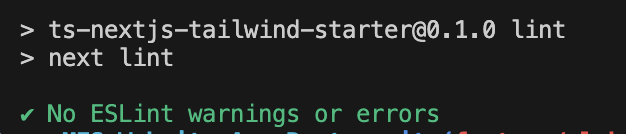
\includegraphics[width=0.95\textwidth]{lint_output.png}
  \caption{ESLint ouput.}
  \label{fig:lint-output}
\end{figure}
Linting runs on all code, so this means 100\% of the lines of code are compliant.

The following shows code coverage of Jest tests in the MES repo. It includes code not written by the Capstone team. Code coverage is a measure of how well the codebase is tested, and it helps identify areas
that may require additional testing. 
\begin{figure}[htbp]
  \centering
  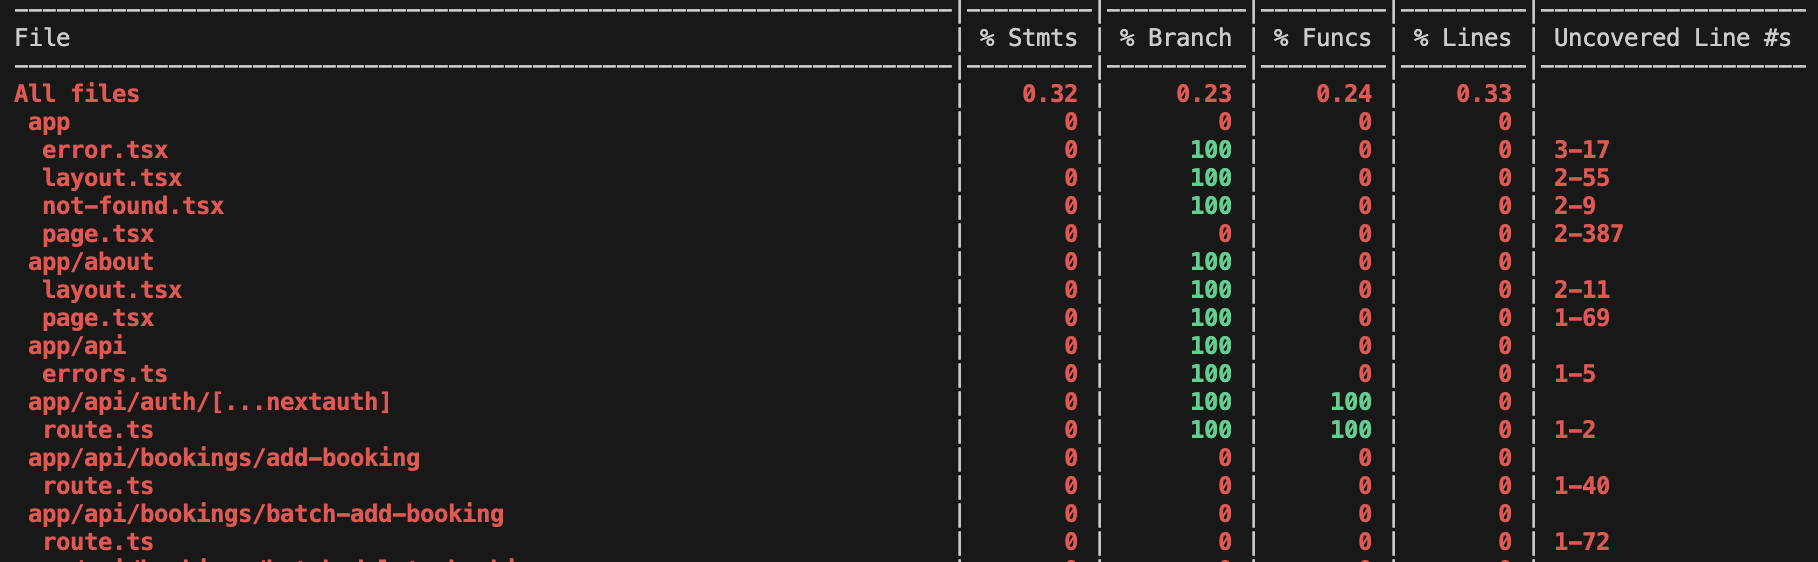
\includegraphics[width=0.95\textwidth]{coverage_report.png}
  \caption{Automated test coverage report.}
  \label{fig:coverage-report}
\end{figure}
In general, coverage is very low and suggests a need for more automated testings with Jest in all aspects.

\bibliographystyle{plainnat}
\nocite{*}
\bibliography{../../refs/References}

\newpage{}
\section*{Appendix --- Reflection}

The information in this section will be used to evaluate the team members on the
graduate attribute of Reflection.

\input{../Reflection.tex}

\begin{enumerate}
  \item What went well while writing this deliverable? 
  \item What pain points did you experience during this deliverable, and how
    did you resolve them?
  \item Which parts of this document stemmed from speaking to your client(s) or
  a proxy (e.g. your peers)? Which ones were not, and why?
  \item In what ways was the Verification and Validation (VnV) Plan different
  from the activities that were actually conducted for VnV?  If there were
  differences, what changes required the modification in the plan?  Why did
  these changes occur?  Would you be able to anticipate these changes in future
  projects?  If there weren't any differences, how was your team able to clearly
  predict a feasible amount of effort and the right tasks needed to build the
  evidence that demonstrates the required quality?  (It is expected that most
  teams will have had to deviate from their original VnV Plan.)
\end{enumerate}

\noindent\textbf{Johnny's Reflection:}
\begin{enumerate}

\item One aspect that went well while writing this deliverable was that we already had a well documented Verification and Validation (VnV) Plan. The structure and testing strategies described in the plan helped guide the organization of the report and made it easier to document the verification activities that were performed.

\item One challenge was that testing was not always at the forefront of our development priorities while building the system. As a result, gathering and organizing the evidence for verification required additional effort near the end of development. We resolved this by reviewing our implemented tests, automated checks, and development history to ensure that all verification activities were properly documented.

\item Most parts of this document stem from a combination of both client and peer feedback. During development, we frequently discussed features and workflows with peers, while during verification and validation we communicated with clients to confirm that the implemented functionality met their expectations. Some sections, such as implementation details and automated testing descriptions, were based primarily on internal development practices rather than external feedback.

\item There were not many differences between the planned and executed VnV activities, particularly for functional verification. The system workflows were relatively straightforward and well defined, which allowed us to follow the original plan closely. Minor adjustments occurred as implementation progressed, but the overall testing strategy remained consistent with the plan. In future projects, similar alignment could be anticipated when requirements and workflows are clearly defined early in development.

\end{enumerate}

\end{document}